%%% Dashboard Implementation
%%%%%%% Wording: ⏳
%%%%%%% Styling: ⏳
%%%%%%% References: ⏳
%%%%% Grammar: ⏳
%\todo{This chapter describes the implementation of the analytical dashboard using Dash and Plotly.}
%\todo{Tools and technologies used - Dash, Plotly, Python, PostgreSQL, SQLAlchemy, Pandas, Mantine Dash Components etc.}
%\todo{Describe async loops for data fetching and Dash background callbacks, f*cking issues with diskcache & DiskcacheManager issues with SQLIte concurrent connections, dscribe how we tried for 12hours straight to fix it and switch to celery + redis for async tasks but then switched back to diskcache with one-liner fix, fml}
%\todo{Describe DB query management - QueryDefinition, QueryRegistry, QueryManger, QueryParameter and other internal classes}
%\todo{Describe additional simple FS query caching mechanism}
%\todo{Describe process of implementing individual dashboard sections, structure and most importantly the chosen visualizations/presentation of data}
%\todo{Defend why we didn't go for deployment to cloud – sorry not sorry I'm not a lunatic, hate Python env and deployment issues}
%\todo{Final dashboard presentation and features}
%\todo{Next steps and missing features and future improvements we would do if we had more time}
%%% --------------------------------------------------------------
\chapter{Dashboard Implementation}
\label{ch:dashboard-implementation}

This chapter describes the implementation of a prototype analytical dashboard that visualizes the key findings from our analysis.
Using Dash and Plotly\footnote{Dash is a Python web application framework that enables the creation of interactive web applications using Plotly visualizations\cite{plotly_dash_plotly_com}.},
we developed a local development prototype that demonstrates how the analytical insights could be presented in an interactive format.
The implementation focused on efficient data querying, caching strategies for development, and handling asynchronous operations in Python.

The chapter details our technical approach, the challenges encountered during implementation (particularly with callback caching and async handling), and our solutions to these challenges.
While not intended for production deployment, the prototype successfully demonstrates the potential of our analytical findings in an interactive format.

%%% Section: Development Approach
%%% --------------------------------------------------------------
\begin{section}{Development Approach}
	\label{sec:implementation-development-approach}

	The implementation phase focused on transforming the analysis results from Chapter~\ref{ch:data-analysis-and-results} into an interactive dashboard prototype.
	Our approach prioritized rapid development and effective visualization of our analytical findings.

	\begin{subsection}{Development Goals}
		\label{subsec:implementation-development-approach-goals}

		The primary goal was to create a functional prototype dashboard that could effectively present our analysis results in an interactive format.
		Specifically, we aimed to:
		\begin{itemize}
			\item Demonstrate key findings through interactive visualizations
			\item Implement basic filtering capabilities for data exploration
			\item Create a responsive interface that handles data operations efficiently
			\item Establish a foundation for visualizing festival transaction data
		\end{itemize}

	\end{subsection}

	\begin{subsection}{Technology Selection}
		\label{subsec:implementation-development-approach-technology}

		The dashboard was build using Dash and Plotly, chosen primarily for their familiarity from prior personal experience in academic field and their great capability for rapid prototyping.
		The technology stack included:

		\begin{itemize}
			\item Dash \& Plotly for the core dashboard framework
			\item Dash Mantine Components\cite{sv_snehilvj_dash_mantine_components} for enhanced UI elements
			\item PostgreSQL\cite{tpgdg_17_postgresql_17_a4_pdf} for local data storage
			\item Python for dashboard backend
		\end{itemize}

		This stack was chosen specifically for prototyping, with Dash and Plotly providing a good balance of functionality and development speed based on our previous experience using these tools in university projects.
		Mantine Components were added to enhance the visual presentation without incurring significant additional development costs.

	\end{subsection}

	\begin{subsection}{Local Development Focus}
		\label{subsec:implementation-development-approach-local}

		The dashboard was developed exclusively for local deployment, focusing on demonstrating analytical capabilities rather than production readiness.
		This decision was influenced by several factors:

		\begin{itemize}
			\item The prototype nature of the implementation
			\item Complexity of Python async handling and production requirements
			\item Deployment challenges with Python environments
			\item Focusing on demonstrating analytical insights rather than production features
		\end{itemize}

	\end{subsection}
\end{section}

%%% Section: Core Architecture
%%% --------------------------------------------------------------
\begin{section}{Core Architecture}
	\label{sec:implementation-core-architecture}

	The dashboard's architecture was designed to handle data efficiently during development, with a particular focus on query management and caching strategies.

	\begin{subsection}{Query Management System}
		\label{subsec:implementation-core-architecture-query-management}

		To manage database interactions efficiently, we implemented a simple \textbf{Query Management System} to handle loading data from our SQL database.
		It consisted of several key components:

		\begin{itemize}
			\item \textbf{QueryDefinition}: Defines query structure and parameters
			\item \textbf{QueryRegistry}: Maintains registered queries
			\item \textbf{QueryManager}: Handles query execution and caching
			\item \textbf{QueryParameter}: Defines parameter types and validation
		\end{itemize}

%		FIXME: autoref with lst:/listing: doesn't work
		The following example in~\autoref{lst:dashboard-implementation-query-management} demonstrates the query registration process:

		\begin{listing}[H]
			\caption{Query Management Example}
			\begin{minted}[breaklines]{python}
query_manager.registry.register_query(
    QueryDefinition(
        name="sankey_diagram",
        sql=QueryManager.process_sql_query("""
            SELECT * FROM get_sankey_diagram_data(:date_from$1, :date_to$2)
        """),
        parameters=[
            QueryParameter("date_from", datetime.datetime),
            QueryParameter("date_to", datetime.datetime)
        ],
        default_data="FSCacheDefault"  # Enables local CSV caching
    )
)
			\end{minted}
			\label{lst:dashboard-implementation-query-management}
		\end{listing}
	\end{subsection}

	\begin{subsection}{Dual Caching Strategy}
		\label{subsec:implementation-core-architecture-caching}

		For the purpose of optimizing the development process, our implementation utilizes two caching mechanisms that are complementary to one another.

		\begin{subsubsection}{Query Result Caching}
			\label{subsubsec:implementation-core-architecture-query-cache}

			To speed up development iterations, we implemented a file-based caching system that stores query results as CSV files.
			This prevented redundant database queries during development:

			\begin{listing}[H]
				\caption{Query Result Caching Implementation}
				\begin{minted}[breaklines]{python}
def execute_query(self, query_name: str, parameters: Dict[str, Any], or_query_def: Optional[QueryDefinition]):
    query_key = self.get_query_key(query_name, parameters)

    if query_def.default_data == "FSCacheDefault":
        try:
            # Read from local CSV cache
            file_path = os.path.join(os.getcwd(), "dashboard_app", "cached-queries", f"{query_key}.csv")
            csv = pd.read_csv(file_path)
            return csv
        except Exception:
            pass

    # Execute database query if cache miss
    result = self._execute_db_query(query_def, parameters)

    # Cache result for future use
    try:
        os.makedirs(os.path.join(os.getcwd(), "dashboard_app", "cached-queries"), exist_ok=True)
        df.to_csv(os.path.join(os.getcwd(), "dashboard_app", "cached-queries", f"{query_key}.csv"), index=False)
    except Exception as e:
        print(f"Failed to save query {query_name} to cache: {e}")

    return result
				\end{minted}
				\label{lst:dashboard-implementation-query-cache}
			\end{listing}
		\end{subsubsection}

		\begin{subsubsection}{Background Callback Caching}
			\label{subsubsec:implementation-core-architecture-callback-cache}

			For handling Dash callbacks, we implemented a background caching mechanism using diskcache:

			\begin{listing}[H]
				\caption{Background Callback Cache }
				\begin{minted}[breaklines]{python}
def create_callback_cache(callback_id: str):
    cache_dir = os.path.join(os.path.dirname(__file__), f'dash_cache_{callback_id}')
    cache = diskcache.Cache(
        directory=cache_dir,
        size_limit=3e9,
        eviction_policy='least-recently-used',
    )

    return dash.DiskcacheManager(
        cache,
        cache_by=[
            lambda: launch_uid,
            lambda: callback_id
        ],
        expire=300
    )
				\end{minted}
				\label{lst:dashboard-implementation-callback-cache}
			\end{listing}

			This implementation evolved through several iterations as we encountered scaling challenges, detailed in the~\autoref{sec:implementation-technical-challenges}~section.
		\end{subsubsection}

		\begin{subsection}{Dashboard Structure}
			\label{subsec:implementation-core-architecture-structure}

			The dashboard's structure mirrors the analysis sections from Chapter~\ref{ch:data-analysis-and-results}, with dedicated sections for:

			\begin{itemize}
				\item \textbf{Cashflow and Revenue Analysis},
				\item \textbf{Performance Analysis},
				\item \textbf{Beverage Consumption Analysis}
				\item and \textbf{Customer Analysis}.
			\end{itemize}

			Each section implements background callbacks for data loading and filtering, using our dual caching strategy to maintain responsiveness during development.

			For each section, a separate file was created, containing the layout and callback definitions for the section.
			The main dashboard file then imports these sections and combines them into a single layout.

			This approach allowed for better code organization and easier development of individual sections.
		\end{subsection}
	\end{subsection}
\end{section}

%%% Section: Technical Challenges and Solutions
%%% --------------------------------------------------------------
\begin{section}{Technical Challenges and Solutions}
	\label{sec:implementation-technical-challenges}

	The implementation process encountered several significant technical challenges, primarily centered around asynchronous operations and callback caching in Python.
	These challenges and their solutions significantly influenced the overall development approach and the outcome of the dashboard prototype.

	\begin{subsection}{Asynchronous Handling Challenges}
		\label{subsec:implementation-technical-challenges-async}

		Coming from a JavaScript/TypeScript background, where asynchronous programming is relatively straightforward\cite{node.js_asynchronous_work_javascript_asynchronous_programming_and_callbacks}, Python's async implementation presented several challenges.
		The main difficulties arose in implementing background tasks for the dashboard's filtering capabilities and data loading operations.

		The initial implementation of background callbacks followed the Dash documentation\cite{plotly_dash_plotly_com_background_callbacks}:

		\begin{listing}[H]
			\caption{Initial Background Callback Implementation}
			\begin{minted}[breaklines]{python}
@callback(
    Output("graph-container", "children"),
    Input("date-picker", "value"),
    background=True,
    manager=background_callback_manager
)
def update_graph(selected_date):
    # Long-running data processing
    df = process_data(selected_date)
    return create_graph(df)
			\end{minted}
			\label{lst:dashboard-implementation-initial-callback}
		\end{listing}

		This approach worked well for individual callbacks but revealed limitations as the dashboard grew in complexity.
	\end{subsection}

	\begin{subsection}{Callback Caching Evolution}
		\label{subsec:implementation-technical-challenges-caching}

		The evolution of our callback caching solution went through several iterations, each addressing specific challenges:

		\begin{subsubsection}{Initial Implementation}
			\label{subsubsec:implementation-technical-challenges-caching-initial}

			Following Dash documentation\cite{plotly_dash_plotly_com_background_callbacks}, we initially implemented a single DiskcacheManager:

			\begin{listing}[H]
				\caption{Initial Cache Manager Setup}
				\begin{minted}[breaklines]{python}
cache = diskcache.Cache(directory=CACHE_DIR)
background_callback_manager = dash.DiskcacheManager(
    cache,
    expire=300
)
				\end{minted}
				\label{lst:dashboard-implementation-cache-initial}
			\end{listing}

			This implementation led to cache key collisions, where callbacks with identical inputs were cached using the same key, resulting in incorrect cached data being returned.
		\end{subsubsection}

		\begin{subsubsection}{First Solution Attempt}
			\label{subsubsec:implementation-technical-challenges-caching-first}

			To address cache key collisions, we implemented unique DiskcacheManager instances for each callback:

			\begin{listing}[H]
				\caption{Unique Cache Managers Per Callback}
				\begin{minted}[breaklines]{python}
def create_callback_manager(callback_id):
    return dash.DiskcacheManager(
        cache,
        cache_by=[
            lambda: launch_uid,
            lambda: callback_id
        ]
    )
				\end{minted}
				\label{lst:dashboard-implementation-cache-unique}
			\end{listing}

			This solution worked well for individual dashboard sections but revealed scalability issues when combining all sections.
		\end{subsubsection}

		\begin{subsubsection}{Scaling Challenges}
			\label{subsubsec:implementation-technical-challenges-caching-scaling}

			As the number of callbacks increased, we encountered SQLite concurrent connection issues.
			The local SQLite database used by DiskcacheManager\cite{gj_diskcache} couldn't handle multiple concurrent connections effectively, causing the dashboard to crash during loading.

			After an unsuccessful 12-hour attempt to implement a Celery\cite{celery_getting_started_introduction}~\&~Redis\cite{redis_latest} solution
			\footnote{
				Celery is a distributed task queue that allows for background task execution, while Redis is an in-memory data structure store used as a database, cache, and message broker\cite{reintech_blog_combining_celery_redis_caching_task_queuing}.
			},
			we opted for a development-focused workaround:

			\begin{listing}[H]
				\caption{Final Cache Implementation}
				\begin{minted}[breaklines]{python}
def create_isolated_cache_manager(callback_id):
    # Create separate SQLite database per callback
    cache_dir = os.path.join(
        os.path.dirname(__file__),
        f'dash_cache_{callback_id}'
    )
    cache = diskcache.Cache(
        directory=cache_dir,
        size_limit=3e9,
        eviction_policy='least-recently-used'
    )

    return dash.DiskcacheManager(
        cache,
        cache_by=[
            lambda: launch_uid,
            lambda: callback_id
        ],
        expire=300
    )
				\end{minted}
				\label{lst:dashboard-implementation-cache-final}
			\end{listing}

			While this solution is not production-ready, it effectively solved our development needs by preventing concurrent SQLite connection issues through database isolation.
		\end{subsubsection}

	\end{subsection}
\end{section}

%%% Section: Implementation Results
%%% --------------------------------------------------------------
\begin{section}{Implementation Results}
	\label{sec:implementation-results}

	Despite the technical challenges encountered, the dashboard prototype successfully demonstrates the key findings from our analysis.
	The implementation provides interactive visualizations of the festival transaction data, organized to reflect our analytical approach.

	\begin{subsection}{Dashboard Structure and Visualization}
		\label{subsec:implementation-results-structure}

		\todo{Add screenshots of the dashboard and describe the structure and visualizations}
		The dashboard is structured into four main sections, directly corresponding to our analysis areas from the~\autoref{ch:data-analysis-and-results}:

		\begin{subsubsection}{Cashflow and Revenue Analysis}
			\label{subsubsec:implementation-results-structure-cashflow}

			The Cashflow Analysis section visualizes overall financial and cashflow patterns using Sankey diagrams and breakdown of revenue streams.

			% TODO
			\todo{Better screenshot after finalization}
			\begin{figure}[H]
				\centering
				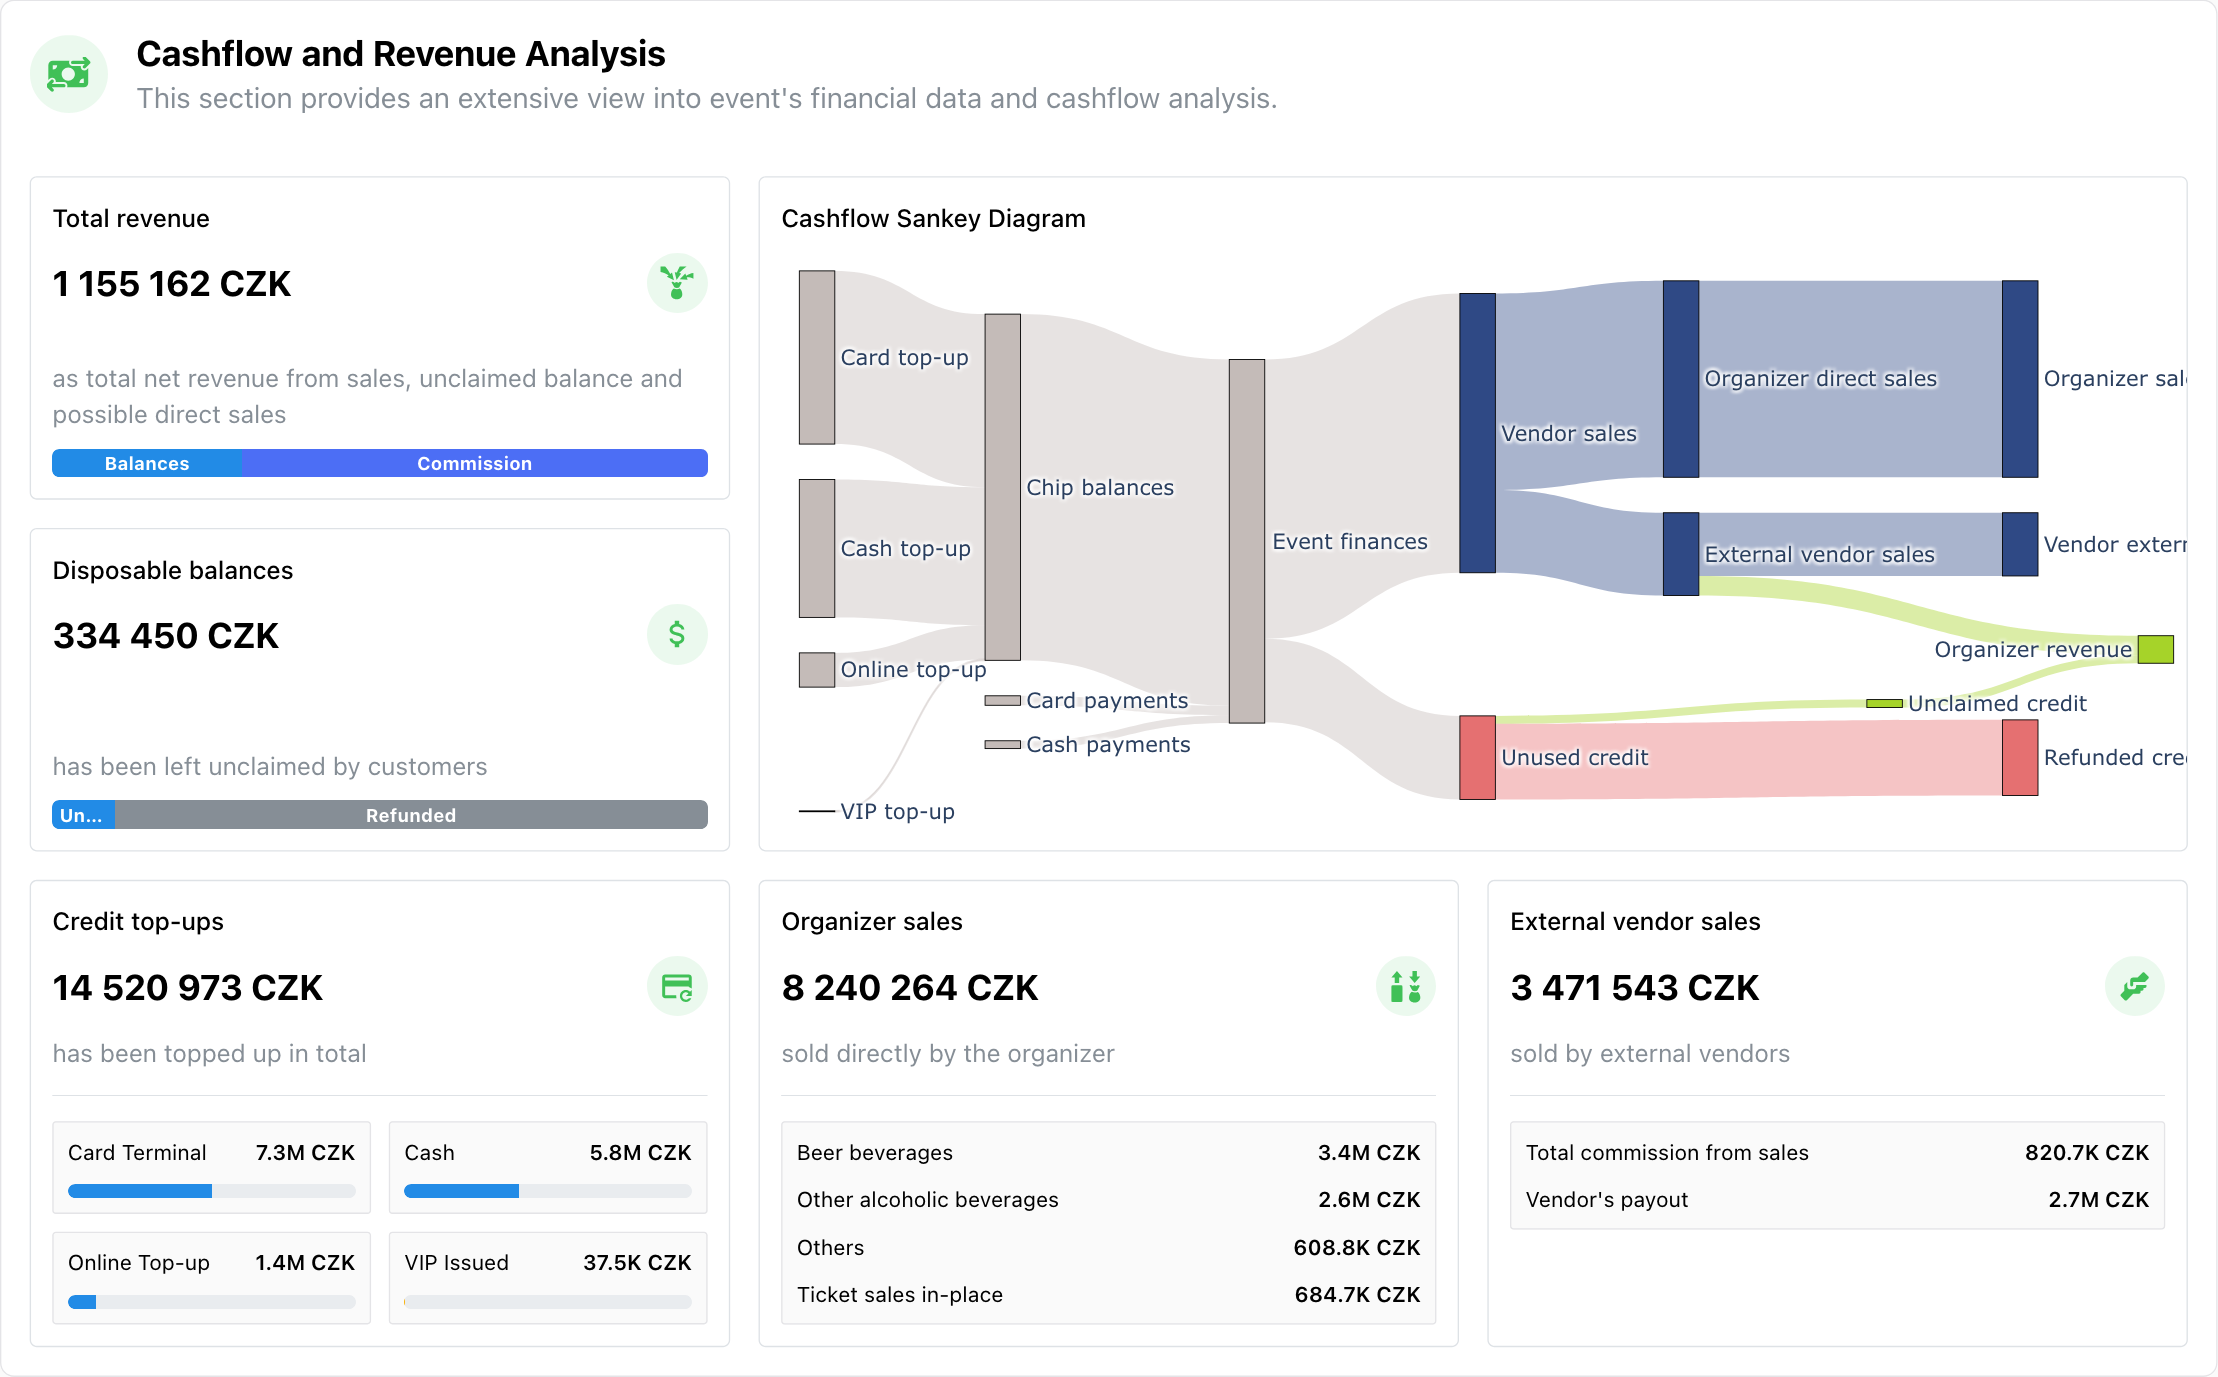
\includegraphics[width=\textwidth]{\ThesisFigures/ui/dashboard-cashflow-section}
				\caption{Cashflow and Revenue Analysis Section}
				\label{fig:dashboard-cashflow-analysis}
			\end{figure}
		\end{subsubsection}

		\begin{subsubsection}{Performance Analysis}
			\label{subsubsec:implementation-results-structure-performance}

			This section focuses on the festival's performance metrics, including mostly transaction processing peaks, capabilities and overall performance.

			% TODO
			\todo{Better screenshot after finalization}
			\begin{figure}[H]
				\centering
				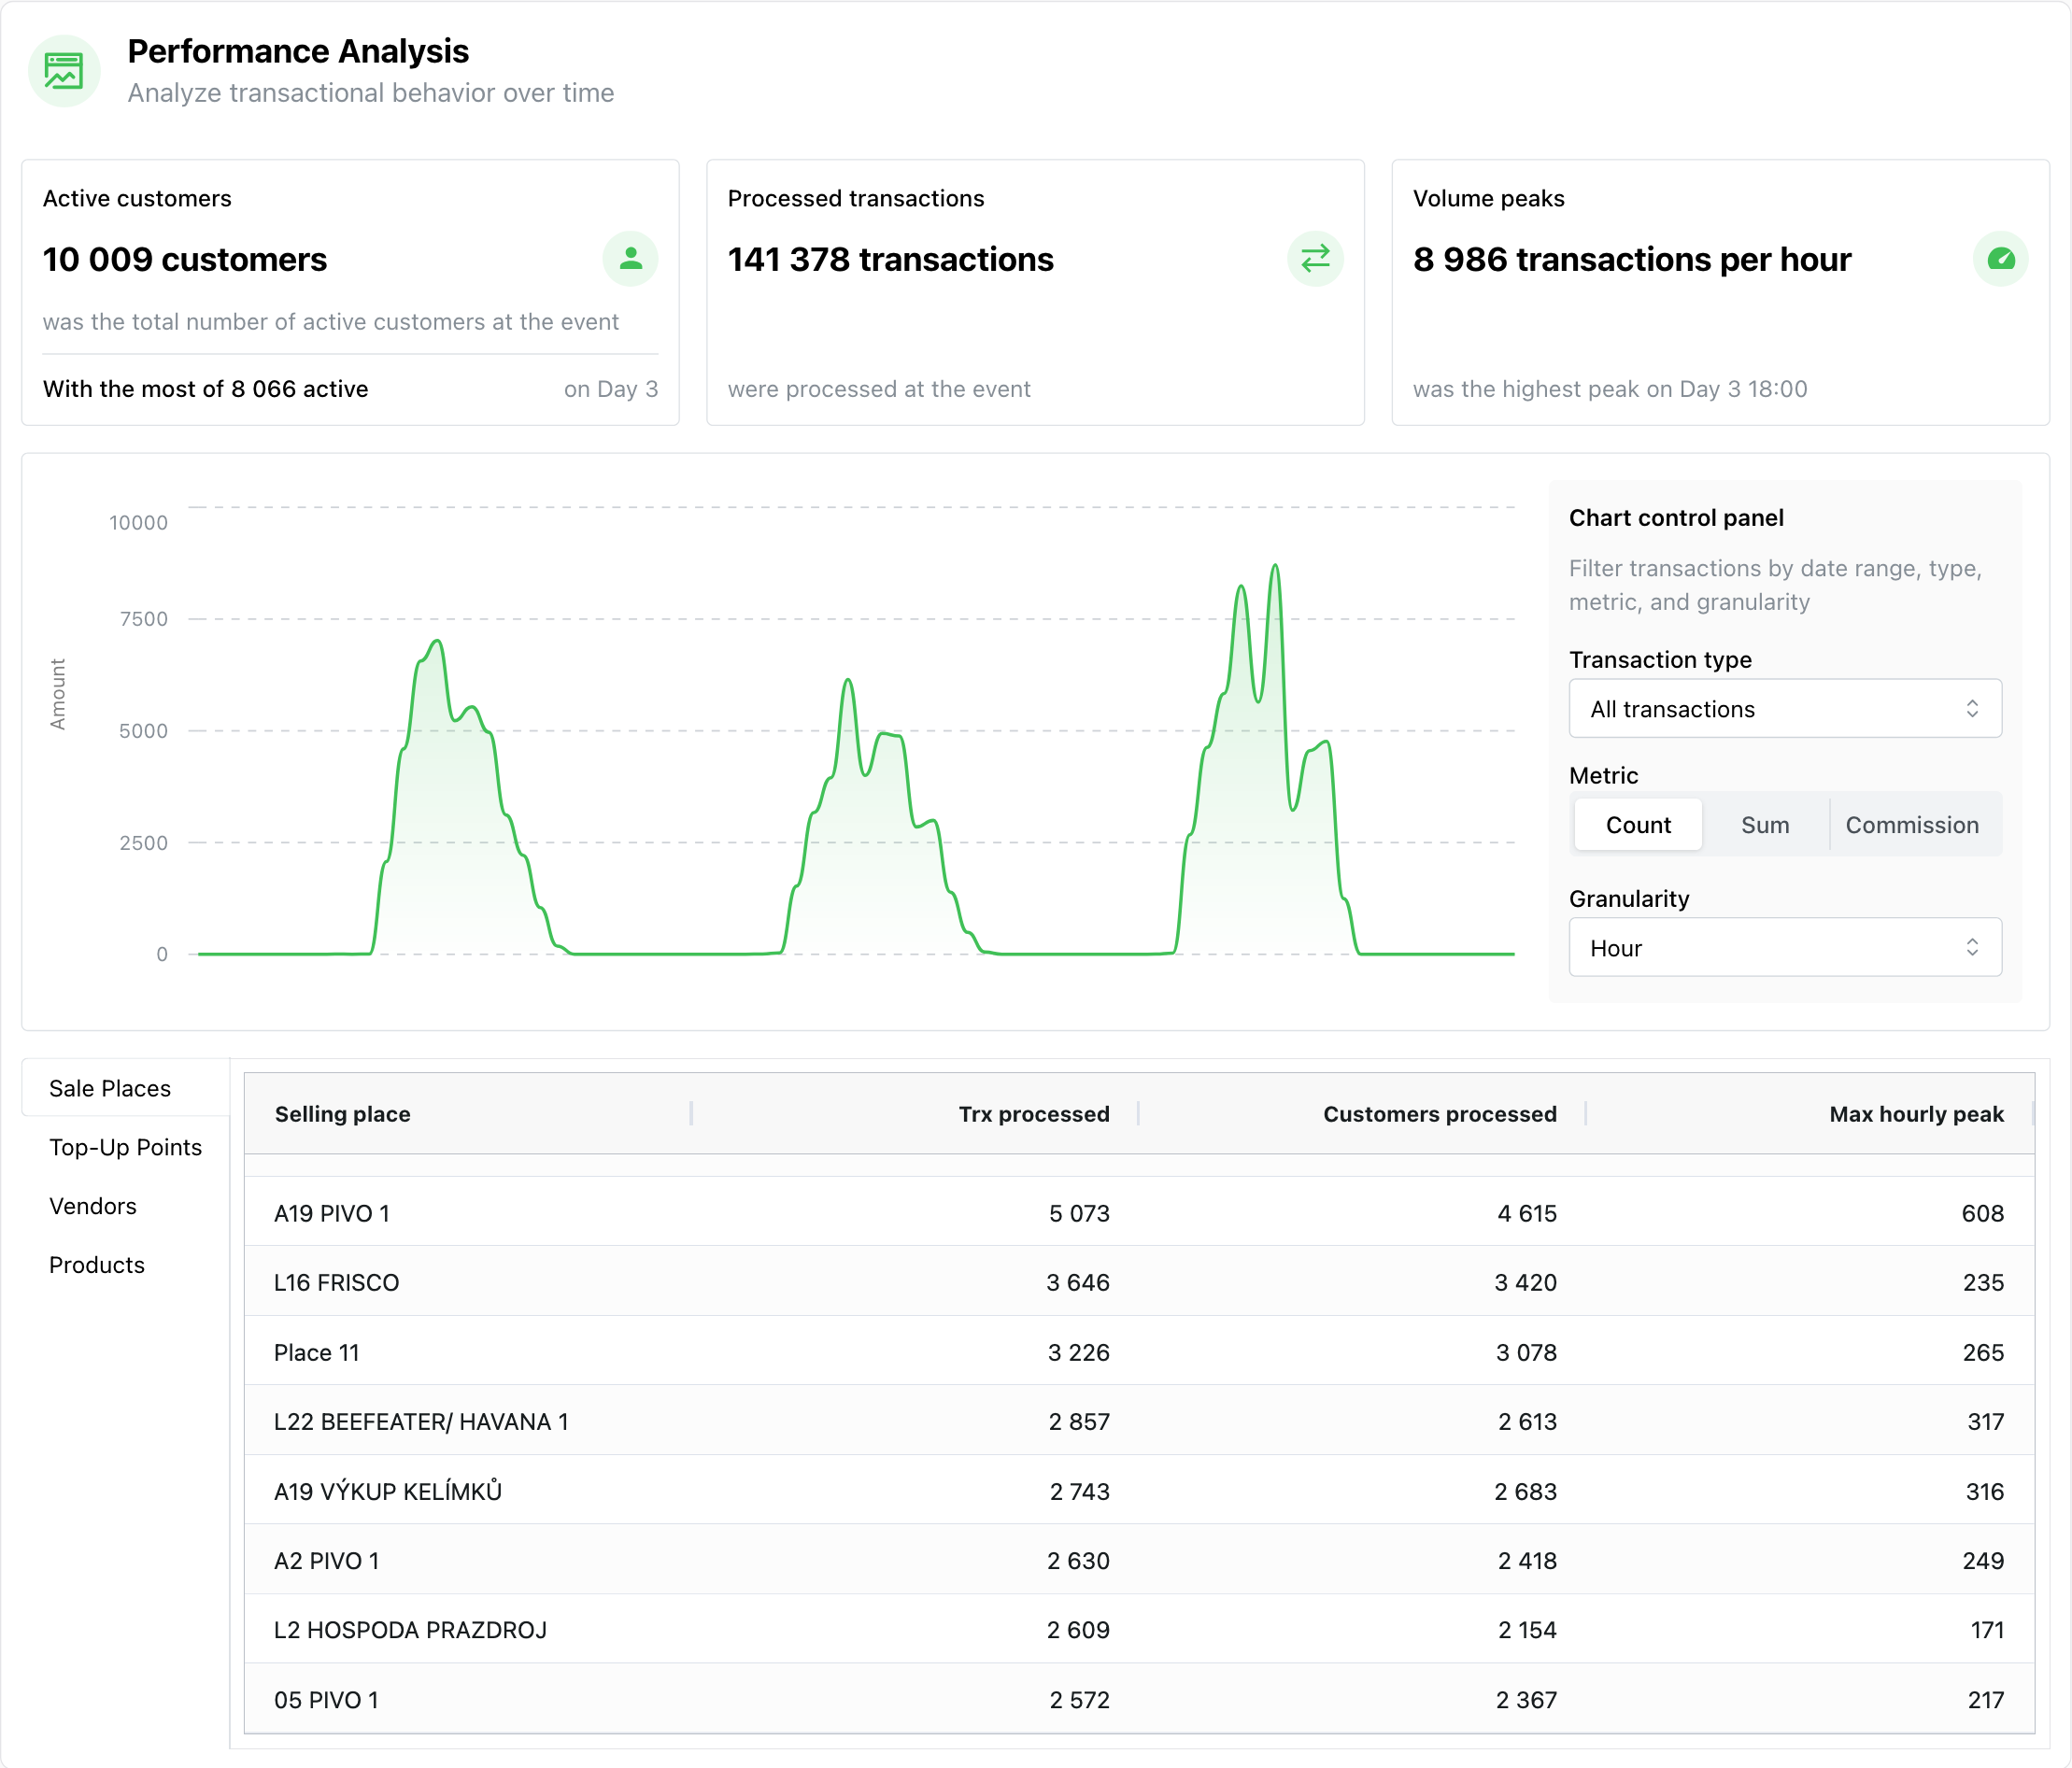
\includegraphics[width=\textwidth]{\ThesisFigures/ui/dashboard-performance-section}
				\caption{Performance Analysis Section}
				\label{fig:dashboard-performance-metrics}
			\end{figure}
		\end{subsubsection}

		\begin{subsubsection}{Beverage Consumption Analysis}
			\label{subsubsec:implementation-results-structure-beverage}

			The Beverage Consumption Analysis section of the dashboard visualizes total beverage statistics, including total consumption amount, returnable cups and most popular beverages.

			% TODO
			\todo{Better screenshot after finalization}
			\begin{figure}[H]
				\centering
				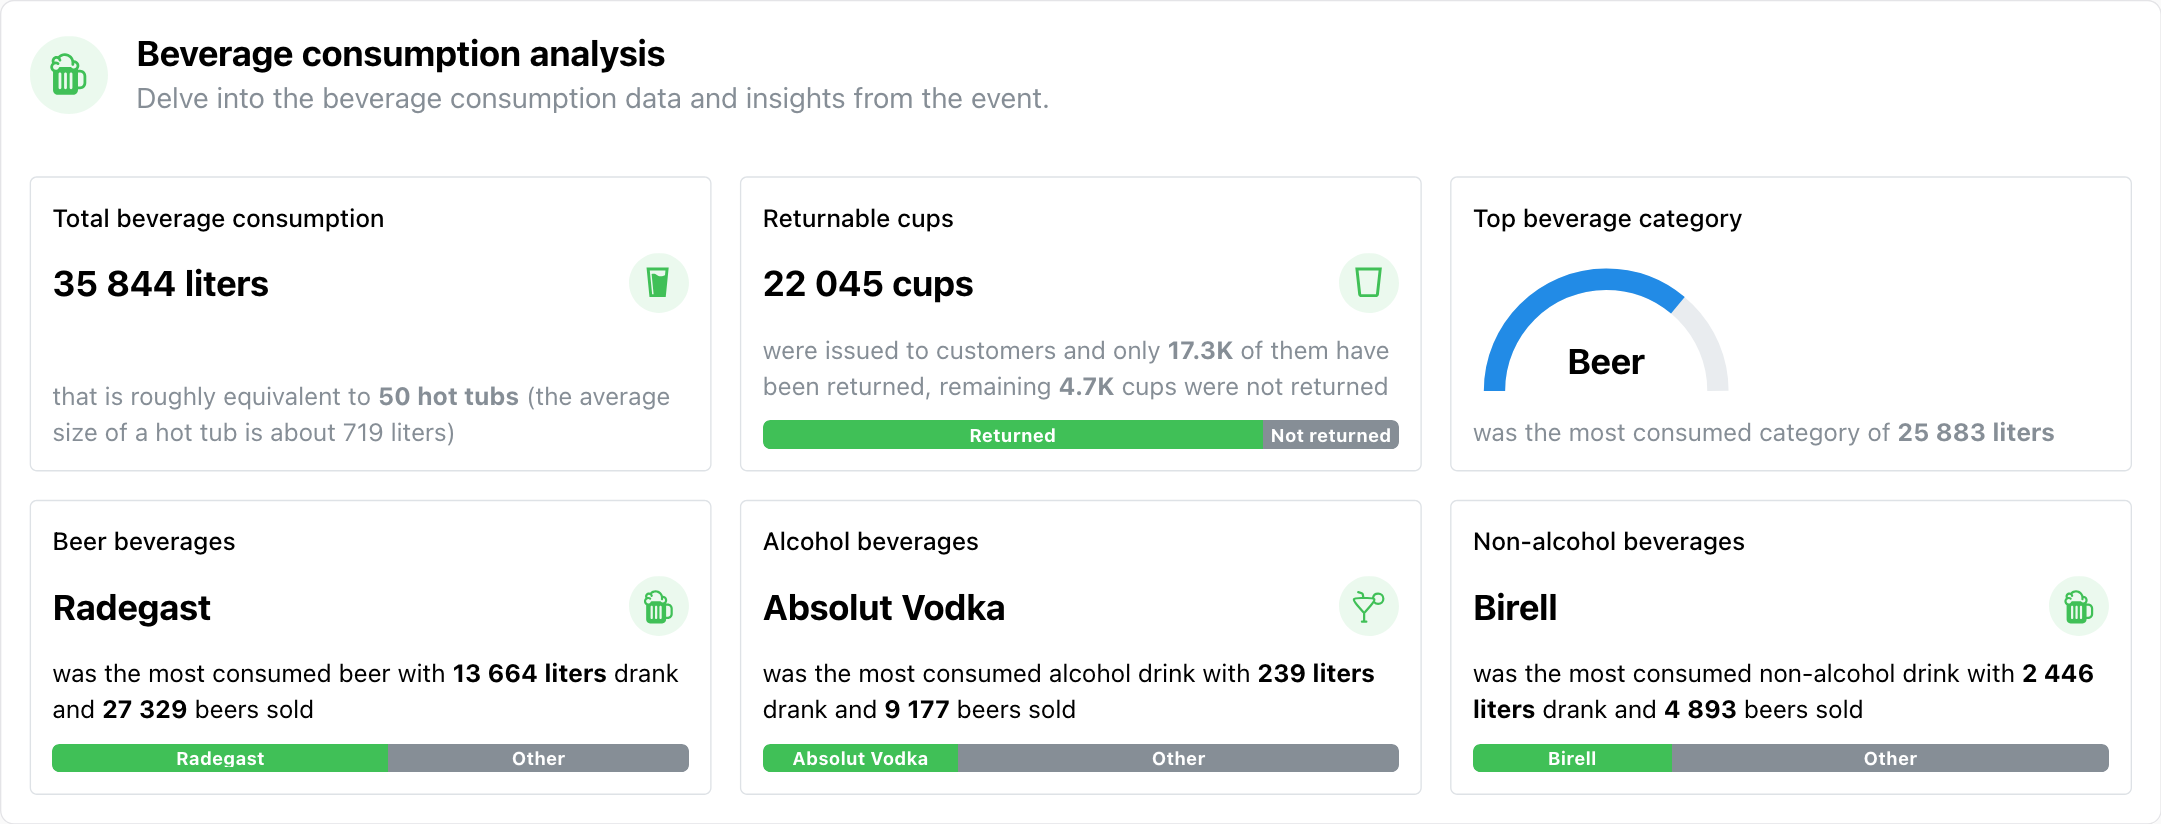
\includegraphics[width=\textwidth]{\ThesisFigures/ui/dashboard-beverage-section}
				\caption{Beverage Consumption Analysis Section}
				\label{fig:dashboard-beverage-sales}
			\end{figure}
		\end{subsubsection}

		\begin{subsubsection}{Customer Analysis}
			\label{subsubsec:implementation-results-structure-customer}

			The Customer Analysis section presents crucial findings about customer segmentation, behavior and sale patterns.
			This section highly benefited from the data analysis performed in the previous chapter and provides a detailed overview of customer demographics and their behavior during the festival.

			% TODO
			\todo{Better screenshot after finalization}
			\begin{figure}[H]
				\centering
				
\includegraphics[width=\textwidth]{\ThesisFigures/ui/dashboard-customer-section}
				\caption{Customer Analysis Section}
				\label{fig:dashboard-customer-behavior}
			\end{figure}
		\end{subsubsection}

		Each section is then located in the overall dashboard layout, where users can navigate between sections and explore the data more interactively than on paper.

		The dashboard benefits from filtering capabilities, allowing users to explore the data based on specific criteria and timeframes.
		For example, the whole dashboard can be filtered to a specific festival day, or a specific time range.
	\end{subsection}

	\begin{subsection}{Technical Implementation Outcomes}
		\label{subsec:implementation-results-technical}
		\todo{Better wording, more details}
		The final implementation achieved several key technical outcomes:

		\begin{itemize}
			\item Effective query management system for handling complex data requests
			\item Dual-layer caching strategy that significantly improved development iteration speed
			\item Workable solution for handling concurrent callback operations in development
			\item Integration of Mantine components for improved visual presentation
		\end{itemize}
	\end{subsection}

	\begin{subsection}{Known Limitations}
		\label{subsec:implementation-results-limitations}
		\todo{Better wording, more details}
		As a prototype implementation, the dashboard has several known limitations:

		\begin{itemize}
			\item Callback caching solution is not suitable for production deployment
			\item Limited to local development environment
			\item Performance optimization focused on development workflow rather than end-user experience
			\item Async handling could be improved with more robust implementation
			\item \todo{Add more limitations we know of}
		\end{itemize}
	\end{subsection}
\end{section}

%%% Section: Future Directions
%%% --------------------------------------------------------------
\begin{section}{Future Directions}
	\label{sec:implementation-future-directions}

	While the current implementation successfully demonstrates our analysis results, several technical improvements could enhance the dashboard:

	\begin{itemize}
		\item Implementation of a more robust callback caching solution using Celery and Redis
		\item Improved async handling with better consideration of Python's async patterns
		\item Optimization of query performance and caching strategies
		\item Enhanced error handling and recovery mechanisms
		\item Deployment to cloud services for broader accessibility and scalability
		\item \todo{Add more future directions we plan(ed) to do}
	\end{itemize}

	These improvements would primarily focus on technical robustness rather than feature expansion, addressing the key limitations identified during development.

	\todo{Describe our previously mentioned personal motivation to do this dashboard and the outcomes of it.}
	\todo{Describe how it already helped us in the work field and enabled us to deliver several updates to our existing dashboard in NFCtron Hub.}
\end{section}
